\documentclass[
	% -- opções da classe memoir --
	12pt,				% tamanho da fonte
	openright,			% capítulos começam em pág ímpar (insere página vazia caso preciso)
	twoside,			% para impressão em verso e anverso. Oposto a oneside
	a4paper,			% tamanho do papel. 
	% -- opções da classe abntex2 --
	%chapter=TITLE,		% títulos de capítulos convertidos em letras maiúsculas
	%section=TITLE,		% títulos de seções convertidos em letras maiúsculas
	%subsection=TITLE,	% títulos de subseções convertidos em letras maiúsculas
	%subsubsection=TITLE,% títulos de subsubseções convertidos em letras maiúsculas
	% -- opções do pacote babel --
	english,			% idioma adicional para hifenização
	french,				% idioma adicional para hifenização
	spanish,			% idioma adicional para hifenização
	brazil,				% o último idioma é o principal do documento
	]{abntex2}


% ---
% PACOTES
% ---

% ---
% Pacotes fundamentais 
% ---
\usepackage{lmodern}			% Usa a fonte Latin Modern
\usepackage[T1]{fontenc}		% Selecao de codigos de fonte.
\usepackage[utf8]{inputenc}		% Codificacao do documento (conversão automática dos acentos)
\usepackage{indentfirst}		% Indenta o primeiro parágrafo de cada seção.
\usepackage{color}				% Controle das cores
\usepackage{graphicx}			% Inclusão de gráficos
\usepackage{microtype} 			% para melhorias de justificação
% ---

% ---
% Pacotes adicionais, usados no anexo do modelo de folha de identificação
% ---
\usepackage{multicol}
\usepackage{multirow}
% ---
	
% ---
% Pacotes adicionais, usados apenas no âmbito do Modelo Canônico do abnteX2
% ---
\usepackage{lipsum}				% para geração de dummy text
% ---

% ---
% Pacotes de citações
% ---
\usepackage[brazilian,hyperpageref]{backref}	 % Paginas com as citações na bibl
\usepackage[alf]{abntex2cite}	% Citações padrão ABNT

\usepackage{float}

\definecolor{verde}{rgb}{0,0.5,0}
\definecolor{cinza}{rgb}{0.95,0.95,0.95}

\usepackage{hyperref}

\usepackage{listings}
\lstset{
  language=[5.0]LUA,
  basicstyle=\ttfamily\small,
  keywordstyle=\color{blue},
  stringstyle=\color{verde},
  commentstyle=\color{red},
  extendedchars=true,
  showspaces=false,
  showstringspaces=false,
  backgroundcolor=\color{cinza},  
  numbers=left,
  numberstyle=\tiny,
  breaklines=true,
  breakautoindent=true,
  captionpos=b,
  xleftmargin=0pt,
}
\pagestyle{empty}


% --- 
% CONFIGURAÇÕES DE PACOTES
% --- 

% ---
% Configurações do pacote backref
% Usado sem a opção hyperpageref de backref
\renewcommand{\backrefpagesname}{Citado na(s) página(s):~}
% Texto padrão antes do número das páginas
\renewcommand{\backref}{}
% Define os textos da citação
\renewcommand*{\backrefalt}[4]{
	\ifcase #1 %
		Nenhuma citação no texto.%
	\or
		Citado na página #2.%
	\else
		Citado #1 vezes nas páginas #2.%
	\fi}%
% ---

% ---
% Informações de dados para CAPA e FOLHA DE ROSTO
% ---
\titulo{Relatório do Trabalho Computacional III}
\autor{Paulo Henrique Rodrigues de Matos e João Pedro Samarino}
\data{24/11/2015}
\instituicao{%
  Universidade de Minas Gerais -- UFMG
  \par
  Faculdade de Arquitetura da Informação
  \par
  Programa de Pós-Graduação}
\tipotrabalho{Relatório técnico}
% O preambulo deve conter o tipo do trabalho, o objetivo, 
% o nome da instituição e a área de concentração 
\preambulo{Relatório para a matéria Eletromagnetismo Computacional}
% ---

% ---
% Configurações de aparência do PDF final

% alterando o aspecto da cor azul
\definecolor{blue}{RGB}{0,0,255}

% informações do PDF
\makeatletter
\hypersetup{
     	%pagebackref=true,
		pdftitle={\@title}, 
		pdfauthor={\@author},
    	pdfsubject={\imprimirpreambulo},
	    pdfcreator={LaTeX with abnTeX2},
		pdfkeywords={Eletromagnetismo Computacional}{Transformador}{Maquinas},
		colorlinks=true,       		% false: boxed links; true: colored links
    	linkcolor=blue,          	% color of internal links
    	citecolor=blue,        		% color of links to bibliography
    	filecolor=magenta,      		% color of file links
		urlcolor=blue,
		bookmarksdepth=4
}
\makeatother

\renewcommand\lstlistingname{Script}
% --- 

% --- 
% Espaçamentos entre linhas e parágrafos 
% --- 

% O tamanho do parágrafo é dado por:
\setlength{\parindent}{1.3cm}

% Controle do espaçamento entre um parágrafo e outro:
\setlength{\parskip}{0.2cm}  % tente também \onelineskip

% ---
% compila o indice
% ---
\makeindex
% ---

% ----
% Início do documento
% ----
\begin{document}

% Seleciona o idioma do documento (conforme pacotes do babel)
%\selectlanguage{english}
\selectlanguage{brazil}

% Retira espaço extra obsoleto entre as frases.
\frenchspacing 

% ----------------------------------------------------------
% ELEMENTOS PRÉ-TEXTUAIS
% ----------------------------------------------------------
% \pretextual

% ---
% Capa
% ---
\imprimircapa
% ---

% ---
% Folha de rosto
% (o * indica que haverá a ficha bibliográfica)
% ---

% ---

% ---
% Anverso da folha de rosto:
% ---


% ---

% ---
% inserir lista de ilustrações
% ---
\pdfbookmark[0]{\listfigurename}{lof}
\listoffigures*
\newpage
% ---

% ---
% inserir lista de tabelas
% ---
\pdfbookmark[0]{\listtablename}{lot}
\listoftables*
\cleardoublepage
% ---



% ---
% inserir o sumario
% ---
\pdfbookmark[0]{\contentsname}{toc}
\tableofcontents*
\cleardoublepage
% ---


% ----------------------------------------------------------
% ELEMENTOS TEXTUAIS
% ----------------------------------------------------------
\textual

% ----------------------------------------------------------
% Introdução (exemplo de capítulo sem numeração, mas presente no Sumário)
% ----------------------------------------------------------
\chapter[Transformador]{Transformador}

\section{Analítica}

No trabalho é apresentado o modelo de um transformador em partes, primeiro o transformador ideal logo em seguida o real com suas imperfeições. Inicialmente no transformador é requerido no item (1.2.5) o calculo das correntes em relação ao numero de espiras de cada lado do transformador, o mesmo pode ser visualizado abaixo.

No transformador ideal temos
$$P_{p} = P_{s}$$
$$\alpha = \frac{V_{p}}{V_{s}} = \frac{N_{p}}{N_{p}}$$
$$V_{p} \times I_{p} = V_{s} \times I_{s} \rightarrow \frac{V_{p}}{V_{s}} = \frac{I_{s}}{I_{p}}$$
logo
$$\alpha = \frac{N_{p}}{N_{s}} = \frac{I_{s}}{I_{p}}$$

Na segunda parte do trabalho o mesmo requer o calculo analítico de $R_{p}$
e $L_{m}$ baseadas na geometria do problema. Para fazer esses cálculos assumimos algumas coisa , são elas , um valor médio do campo magnético para calcular a indutância ($L_{m}$
), também assumimos que a profundidade de penetração nesse caso é desconsiderável. 
Temos que lembrar que esses valores calculados servem somente como uma referencia , pois não oferecem nenhuma precisão em relação ao modelo do problema , abaixo podemos ver os valores encontrados:

$$S = l \times c = 0.00143541\mathrm{m^{2}}$$
$$\lambda = n . \phi $$
$$\phi = \int_S \! f(x) \, \mathrm{d}s$$

Assumimos o  $\vec B$ normal à superficie 

$$\lambda = n . \phi = 1,2274 \times 0,001435 \times 260 = 0,4580$$
$$L_{m} = \frac{\lambda}{I} = \frac{0,4580}{0,1578} = 2,9158  \mathrm{H}$$

A superficie do $\mathrm{AWG18} = 8,23 \times 10^{-7} \mathrm{m^2}$ e a resistividade $\rho = 1,72 \times 10^{-8} \mathrm{m.\Omega}$. Em uma volta da bobina temos 0,0824m de fio.


Pela Segunda lei de Ohm temos
$$ R_{p} = \frac{\rho . l}{S} = \frac{1,72 \times 10^{-8} \times 21,424}{8,23 \times 10^{-7}} = 0,44 \mathrm{\Omega} $$

\section{Computacional}

\subsection{Ponto de operação}
Nessa analise foi feito algumas adições no modelo proposto, foi adicionado às condições de contorno e os valores específicos do problema. Foi colocado no problema condições de dirichlet, pois estamos modelando somente o transformador sem o ambiente externo, os materiais foram adicionados de acordo com a imagem na apresentação do trabalho onde mostrava estas características, os mesmos foram adicionados da biblioteca nativa do FEMM.
Na figura \ref{fig:simulacao_inicial} podemos ver o modelo já simulado com as condições estabelecidas inicialmente.

\begin{figure}[H]
    \centering
    \includegraphics[width=15cm]{img/simulacao_traf.png}
    \caption{Condição inicial da simulação}
    \label{fig:simulacao_inicial}
\end{figure}


A primeira analise proposta foi em relação ao ponto de operação do problema, se desejava ter na entrada 127Vrms e estudar o transformador em aberto, ou seja, quando a corrente no secundário é (0)A . Para fazer isto modificamos a corrente no primário ate achar a tensão de operação, lembrando que o FEMM trabalha só com corrente como condição inicial e a tensão é resultado da mesma, então para achar a tensão de 127V no primário, primariamente tivemos que variar a corrente, começamos com o valor de 0,1A e com o valor do resultado calculávamos a tensão RMS resultante. Como o valor de (0,1)A já se obtém uma tensão em torno de 80V, então sabíamos que o valor não era muito distante, então testamos um valor 50\% maior 0.15A o que resultou algo em torno de 126V, já esperávamos um valor próximo devido o tipo de circuito do transformador real, depois testamos o valor de 0.16A o que resultou em um pouco maior . Para refinar esse valor utilizamos mais tentativas com passos curtos, por fim obtivemos os valores que estão na figura \ref{fig:valores_pri}.

\begin{figure}[H]
    \centering
    \includegraphics[width=6cm]{img/valores_1.png}
    \caption{Valores no primairo do trafo}
    \label{fig:valores_pri}
\end{figure}

Temos que nos lembrar de que o valor que o FEMM nos informa é o valor complexo da tensão, então Tensão RMS = $\sqrt{42,3677^2+174,575^2}/\sqrt{2} =  127,026\mathrm{V}$.

Um valor bem próximo do que foi pedido, não achamos necessário se obter o valor exato da corrente, pois o erro nesse caso já era bem pequeno.
Com essa especificação  de corrente na entrada temos na figura \ref{fig:valores_sec}  tensão de saída do secundário 

\begin{figure}[H]
    \centering
    \includegraphics[width=6cm]{img/valores_2.png}
    \caption{Valores no secundário do trafo}
    \label{fig:valores_sec}
\end{figure}


Tensão RMS = $\sqrt{14.6412^2+60.4214^2}/\sqrt{2} =  43,96$V
Agora comparando com um transformador ideal temos que a tensão esperada fosse:
 Tensão RMS = $127,026 \times 90/260 = 43,97$V
Isso mostra que a queda de tensão de (Rp) é muito pequena. O desvio para esse caso do transformador para o real é apenas 0,022\%.

\subsection{Estimativa dos parâmetros}

A segunda analise proposta foi em relação a estimativa dos parâmetros do transformador e depois os mesmo serão comparados com o valor do analítico calculado na primeira parte deste trabalho, para isso temos que usar a seguinte condições :
Para estimar  $R_{c}$ e $L_{m}$ consideramos que a queda de tensão sobre eles e igual a do primário , logo temos a seguinte relação :
$$\frac{1}{Z_{t}} = \frac{1}{Z_{r}} + \frac{1}{Z_{l}}$$
E temos que $Z_{r} = R_{c}$

Utilizando essas considerações temos que $Z_{t}$ é o valor informado na figura  \ref{fig:valores_pri}  e tem o valor de:
$Z_{t} =  269,68+ 1111,23J\mathrm{\Omega}$.
O programa também informa a potencia real que tem o valor de 3,32 W (figura  \ref{fig:valores_pri}), com isso podemos determinar  $Z_{c}$, pois o mesmo consome toda a energia real do sistema, para esse caso, então:
$$V = R \times I$$ 
$$P = \frac{V^2}{R} \rightarrow R = \frac{V^2}{P}$$

De forma aproximada temos que:
$$R_{c} = \frac{127,026^2}{3,32} = 4,85 \mathrm{k\Omega}$$

logo $Z_{l} = 1176,7j \mathrm{\Omega}$
$$Z_{l} = \omega jL \rightarrow L_{m} = 1176.7/60  = 19,6\mathrm{H}$$

Para estimar $R_{p}$ temos que saber a queda sobre o mesmo, para isso podemos usar de maneira aproximada a tensão de saída do secundário que o FEMM nos informa na figura \ref{fig:valores_sec}, logo podemos através da relação do transformador ideal  saber a tensão sobre o primário e determinar assim a queda sobre $_R{p}$, essas relações podem ser vistas abaixo: 
$V_{p} = 260/90 \times 43,96 = 126,989$V

Então temos que $V_{rp}$ e dado pela diferença entre tensão de entrada e tensão na bobina ideal $V_{p}$.  $V_{rp} = (127,026 - 126,989) \times \sqrt{2} = 0,0512$V
Logo temos que $R_{p} = 0,0512/0,1571 = 0,33 \Omega$. Podemos reparar que nesse caso usamos só a parte real, ou seja, o ângulo de defasem da tensão e corrente não foi considerado, pois para o calculo de Rp os mesmos são irrelevantes.

Comparando esses valores com a parte analítica podemos notar então que os valores tiveram certa faixa de incerteza, está foi gerada pelas considerações analíticas feitas na geometria.  E a aproximação feita no item (1.3.2) é valida, pois os valores de Rp e Lsp são muito pequenos, sendo nesse caso uma boa aproximação para o problema em questão.

\subsection{Perdas no transformador}
Nesta ultima analise da primeira parte do trabalho, se deseja mostrar as perdas no transformador em relação à frequência e a condutividade do núcleo, para que pudéssemos obter uma melhor analise utilizamos de script feito em lua que podem ser visto no  apêndice \ref{ch:script_lua}. 

\subsubsection{Perda por variação de frequência}
A primeira analise dessa parte foi em relação à perda por variação de frequência, para isso inicialmente estudamos neste modelo quais os fenômenos estavam relacionados a esta variação, concluímos que quando variamos a frequência devido à superfície de penetração o valor do campo magnético se alterava no interior do transformador, esse fenômeno já era previsto, por isso fomos mais cautelosos ao estuda-lo. Sabendo disso além de coletar pontos de perdas coletamos os valores de B em um ponto médio do transformador para que pudéssemos estudar o fenômeno da perda associado ao fato da variação do campo.

Através dessa amostra (tabelas \ref{tab:p_f_i} \ref{tab:p_f_ii} \ref{tab:p_f_iii} \ref{tab:p_f_vi}) montamos os seguintes gráficos da perda e do valor de B, os mesmos foram feitos no software R e podem ser na figura \ref{fig:gra_p_f}.

\begin{figure}[H]
    \centering
    \includegraphics[width=10cm]{img/perda_frequencia.png}
    \caption{Gráfico Frequência $\times$ Perda }
    \label{fig:gra_p_f}
\end{figure}

Através do gráfico representado na figura \ref{fig:gra_p_f} vemos a curva real de perda do nosso modelo de transformador, reparamos que a mesma tem uma curva característica que parece ser influenciada por outros fatores além da frequência.

\begin{figure}[H]
    \centering
    \includegraphics[width=10cm]{img/b_frequencia.png}
    \caption{Gráfico |B| $\times$ Frequência }
    \label{fig:gra_b_f}
\end{figure}

Como o gráfico descreve o valor B em relação à frequência, a mesma sofre uma queda, isto é resultado da característica do material e profundidade de penetração.
Podemos pensar que o gráfico da perda por frequência não resultou em algo esperado porem como a perda nesse modelo são quase em sua totalidade gerada no ferro, a equação que modela o mesmo é:

\begin{equation} \label{eq:perda}
  P_{f} = \frac{1}{24} \sigma \omega^2e^2B_{max}^2
\end{equation} 


Podemos notar que a perda também é em função de ($B^2$) então se pode utilizar desse fato para criar um novo gráfico onde o eixo Y será (perda/(campo ao quadrado)), este pode ser visualizado na figura \ref{fig:gra_w_f}

\begin{figure}[H]
    \centering
    \includegraphics[width=10cm]{img/w_frequencia.png}
    \caption{w $\times$ Frequência }
    \label{fig:gra_w_f}
\end{figure}

Nesse gráfico se pode notar que a curva é uma quadrática, o resultado saiu como esperado para o modelo que usamos, e podemos dizer que o mesmo pode ser modelado pela a equação \ref{eq:perda}

\subsubsection{Perda por variação de condutividade}

Para analisarmos a perda em relação à variação da condutividade do núcleo também usamos (Lua), porem utilizamos uma quantidade menor de pontos (71) para modelar, e utilizamos o mesmos pressuposto descrito acima, ou seja, utilizamos medidas de B para uma melhor visualização  e entendimento das características do mesmo. 
Os valores da perdas pode ser visualizado na tabela \label{tab:p_f_vi}

\begin{figure}[H]
    \centering
    \includegraphics[width=10cm]{img/perda_condutividade.png}
    \caption{Perda $\times$ Condutividade}
    \label{fig:gra_p_c}
\end{figure}

No gráfico da figura \ref{fig:gra_p_c} vemos que existe um pico de perda e depois o gráfico segue uma curva com um decaimento mais suave, a condutividade nesse caso como a geometria pode afetar em muitos aspectos o comportamento do sistema e de outras variáveis, como é o caso de B que pode ser visto no gráfico da figura \ref{fig:gra_b_c} 

\begin{figure}[H]
    \centering
    \includegraphics[width=10cm]{img/b_condutividade.png}
    \caption{B $\times$ Condutividade}
    \label{fig:gra_b_c}
\end{figure}


Podemos ver o comportamento de B com a condutividade do metal e percebemos que com o seu aumento o campo em um ponto central decai. 
Podemos ver que a relação da condutividade na equação \ref{eq:perda}  é linear  em relação a perda , porem para visualizar este fato temos então que utilizar dos artifícios que usamos anteriormente, e plotar o novo eixo em (perda/(campo ao quadrado)), na figura \ref{fig:gra_w_c} podemos ver o gráfico  
 
\begin{figure}[H]
    \centering
    \includegraphics[width=10cm]{img/w_condutividade.png}
    \caption{W $\times$ Condutividade}
    \label{fig:gra_w_c}
\end{figure}


A curva plotada sofre certa variação de derivada depois de 20MS/m talvez isto esteja relacionada ao fato de que utilizamos um ponto médio para medir a tendência de B ou possa ser algo em torno do ponto de operação do ferro utilizado ou outro fenômeno que não conseguimos identificar e esteja correlacionado, de qualquer forma, vemos que não sofre alterações bruscas e se aproxima de uma reta, mostrando assim que a analise de B nesse caso é de extrema importância, como mostra a equação acima.


\chapter[Máquinas elétricas trifásicas]{Máquinas elétricas trifásicas}

\section{Movimentação do campo magnético}

Para esta analise, primeiro se deve lembrar  que o campo magnético depende das correntes das boninas do estator, as mesmas  variam com o tempo de acordo com as seguintes equações.

\begin{equation}
	I_{a} = 2 \times \mathrm{cos} (\omega t) 
\end{equation}

\begin{equation}
	I_{b} = 2 \times \mathrm{cos} (\omega t + 120) 
\end{equation}

\begin{equation}
	I_{c} = 2 \times \mathrm{cos} (\omega t + 240) 
\end{equation}

Encontramos essa equações usando como base os valores inicias do arquivo motor.femm 

\begin{equation}
	I_{a} = 2 = 2 \angle 0 
\end{equation}

\begin{equation}
	I_{b} = -1 + 1.732i = 2 \angle 120
\end{equation}

\begin{equation}
	I_{c} =  -1 - 1.732i = 2 \angle 240 
\end{equation}

Com base nisso podemos concluir que o motor esta ligado na sequência A-C-B.

Isso faz com que apareça um campo girante, pois as mesmas, como podemos ver seguem um regime senoidal no tempo, o que faz com que o campo não seja estático e sempre esteja girando, podemos ver melhor esse efeito atreves do vídeo produzido unicamente para este trabalho, o mesmo pode ser acessado por esse \href{https://www.youtube.com/watch?v=nX_oYFQX8Uc}{link}

No vídeo fica claro, que quando colocamos as correntes para variar de maneira senoidal o campo gira em função das fases utilizadas, no caso utilizamos a sequencia (A-C-B), mudando a sequencia poderíamos fazer com que o campo girasse inversamente ao sentido do apresentado no vídeo, o mesmo efeito seria alcançado se a defasagem fosse inversa, ou seja -120 graus. As imagens \ref{fig:trafo_abc} \ref{fig:trafo_acb} exemplificam esse fato.

\begin{figure}[H]
    \centering
    \includegraphics[width=8cm]{img/motor_acb_45.png}
    \caption{Analise do campo gerado pelo estator. Sendo Fase de A = 45 e ligação ACB}
    \label{fig:trafo_acb}
\end{figure}

\begin{figure}[H]
    \centering
    \includegraphics[width=8cm]{img/motor_abc_45.png}
    \caption{Analise do campo gerado pelo estator. Sendo Fase de A = 45 e ligação ABC}
    \label{fig:trafo_abc}
\end{figure}

Temos que lembrar que para esse efeito ocorrer as fases em sequencia devem ter uma defasagem uma em relação a outra de 120 graus, isso garante que o campo sempre esteja girando se as correntes das boninas variarem de maneira senoidal.

Para montarmos este vídeo utilizamos script (LUA), o mesmo pode ser acessado no apêndice \ref{ch:script_lua} . Fizemos dessa maneira a analise para mostras de maneira dinâmica a variação do campo no regime do tempo e identificar possíveis problemas no nosso modelo. O resultado dessas analise saiu como o esperado e não houve nenhuma eventualidade no mesmo.


A Segunda parte deste trabalho consiste em tirar resultados de um modelo de um motor  trifásico montado no FEMM, foram feitas varias analise nesse modelo, alguma dessas foram feitas de maneira que ficasse mais simples o entendimento.


\section{Força e torque sobre o rotor}

Nessa analise, diferente da anterior estamos interessados em sabermos o torque sobre o rotor em um determinado estante de tempo, ou seja, consideramos um campo estático induzido pelas bobinas.

Para o rotor utilizamos uma corrente fixa, e somente uma bobina para ficar mais simples o estudo deste fenômeno, o campo gerado por ela pode ser observada na figura \ref{fig:m_c_b}

\begin{figure}[H]
    \centering
    \includegraphics[width=15cm]{img/motor_campo_bobina.png}
    \caption{Campo Bobina}
    \label{fig:m_c_b}
\end{figure}



Devemos lembrar que a posição do rotor varia sua posição, para que dessa forma se analise o torque sobre o rotor, no entanto o mesmo varia imerso sobre o campo gerado pelo estator. Para fazer essa analise mais uma vez criamos um vídeo que pode ser visualizado por esse \href{https://www.youtube.com/watch?v=PQLGsbMnyD4}{link}

Neste podemos ver que em alguns momentos o campo B se altera, fato que já era esperado, pois existe a interação entre os dois campos mostrados nas imagens acima. Agora para calcularmos o torque exato a cada grau de rotação, utilizamos o calculo de torque do FEMM sobre o rotor para cada grau, para fazermos esse montante de simulações utilizamos um script (LUA) que pode ser acessado no apêndice \ref{ch:script_lua} , este gerou para nos as seguintes tabelas \ref{tab:pr_i}  \ref{tab:pr_ii}  \ref{tab:pr_iii}  \ref{tab:pr_iv}, a mesmo foi transformada em um gráfico atreves do software R, e pode ser visualizado na figura \ref{fig:torque}


\begin{figure}[H]
    \centering
    \includegraphics[width=10cm]{img/torque.png}
    \caption{Torque}
    \label{fig:torque}
\end{figure}

Podemos notar que o maior torque acontece em 0 e 180 graus e tem seu valor nulo em 90 e 270 graus, tal valor já era esperado, pois no momento de maior torque o campo do rotor em relação ao do estator são perpendiculares, e no de menor são paralelos. Este fato pode ser melhor visualizado através das forças exercidas pelo campo sobre a bobina. Para se calcular essa força podemos utilizar a relação de força de Lorentz, que esta na equação \ref{eq:forca_completa}

\begin{equation} \label{eq:forca_completa}
	\vec F = q(\vec E + \vec v \times \vec B)
\end{equation} 

Lembrando que para isso consideramos o campo magnético  dentro do estator constante , o que é uma boa aproximação, então como a força nesse caso sempre terá uma mesma direção para cada bobina , logo para a situação de torque 0 e torque máximo temos as seguintes situações , que podem ser melhor visualizadas nas imagens \ref{fig:motor_max} \ref{fig:motor_nulo}

\begin{figure}[H]
    \centering
    \includegraphics[width=10cm]{img/Motor_forca_max.png}
    \caption{Motor força maxima}
    \label{fig:motor_max}
\end{figure}

\begin{figure}[H]
    \centering
    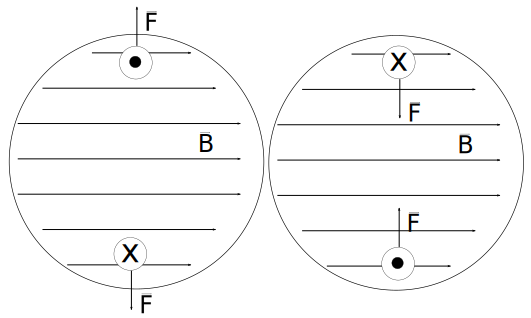
\includegraphics[width=10cm]{img/Motor_forca_min.png}
    \caption{Motor força nula}
    \label{fig:motor_nulo}
\end{figure}


Como podemos ver nas imagens  para  a situação de torque 0 temos as forças se anulando pois são opostas ou tem a mesma direção , para o torque máximo temos a situação onde as forças são somadas e criam um torque máximo , pois são opostas e não  estão sobre o mesmo eixo.

\begin{figure}[H]
    \centering
    \includegraphics[width=15cm]{img/img_090.png}
    \caption{Simulação Torque nulo}
\end{figure}

\begin{figure}[H]
    \centering
    \includegraphics[width=15cm]{img/img_180.png}
    \caption{Simulação Torque máximo}
\end{figure}

\section{Máquinas síncronas}

Com raras exceções, o enrolamento de armadura de uma maquina síncrona localiza-se no estator, e o enrolamento do campo, no rotor, podemos visualizar um esquemático dessa situação na figura \ref{fig:gerador}.

Analisando a figura \ref{fig:gerador} podemos ver que o enrolamento do campo gera apenas um par de polos, o enrolamento da armadura aqui é uma única bobina de N espiras. O rotor é girador por uma força mecânica e tem o sua velocidade de modulo constante. Supõe-se que o enrolamento de armadura esteja em circuito aberto, e portando o fluxo dessa máquina será produzido apenas pelo enrolamento do campo.

Podemos ver o caminho do fluxo na figura \ref{fig:gerador}, analisando a maquina como uma maquina ideal, o fluxo magnético no entreferro é senoidal. A medida que o rotor gira, o fluxo sobre o enrolamento da armadura varia no tempo, produzindo uma tensão senoidal no tempo, essa tensão passa por um ciclo completo a cada revolução do rotor e sua frequência é a mesma que a velocidade do motor. Assim uma máquina síncrona de dois polos deve girar a 3600 rotação por minutos para produção de uma tensão de 60Hz
\begin{figure}[H]
    \centering
    \includegraphics[width=8cm]{img/gerador.png}
    \caption{Diagrama esquemático de um gerador síncrono, pólos salientes, monofásico, dois pólos}
    \label{fig:gerador}
\end{figure}

Podemos ter mais de um pólo em uma maquina síncrona, como podemos ver na figura \ref{fig:gerador_mono_4}. Reparamos que as bobina do campo estão ligado de modo que os polos tenham polaridades alternadas. O enrolamento de armadura consiste agora duas bobinas , $a_{1}$, $-a_{1}$ e $a_{2}$ e $-a_{2}$ ligadas em série pelos seus terminais de conexão. A cada bobina corresponde um comprimento de onda de fluxo. Temos agora dois compelimentos de ondas a cada revolução do rotor. Assim a frequência em Hz sera o dobro da rotação por segundo.

A tensão de uma bobina de uma máquina de múltiplos polos passa por um ciclo completo toda vez que um par de polos passa pela bobina. A frequência elétrica $f_{e}$ gerada por uma maquina de síncrona é  portando\begin{equation}
f_{e} = \frac{pólos}{2} \times  \frac{n}{60} 
\end{equation} onde n é a velocidade mecânica em rotações por minuto.


\begin{figure}[H]
    \centering
    \includegraphics[width=6cm]{img/gerador_mono_4.png}
    \caption{Diagrama esquemático de um gerador síncrono, de pólos
salientes, monofásico, quatro pólos}
    \label{fig:gerador_mono_4}
\end{figure}

Para a construção de uma maquina trifásica , deve ser usado no mínimo três bobinas defasadas de 120 graus elétricos no espaço, podemos ver um esquemático na figura \ref{fig:gerador_a}. Em uma maquina elementar de Quatro pólos, um mínimo de dois conjuntos de bobinas deve ser usados podemos ver o esquemático na figura \ref{fig:gerador_b}.  Em um maquina elementar com múltiplos polos, o numero mínimo de conjuntos de bobina é dado pela metade do números de pólos.
As duas bobinas da figura \ref{fig:gerador_b} são conectadas em series de modo que sua tensões sejam somadas e e as tres fases podem ser ligadas em $Y$ ou em $\Delta$ como na figura  \ref{fig:gerador_c} onde vemos a ligação em $Y$. Uma alternativa possível também é a ligação em paralelo do par de bobinas.

\begin{figure}[H]
    \centering
    \includegraphics[width=6cm]{img/gerador_s.png}
    \caption{Diagrama esquemático de gerador trifásico - dois polo e um enrolamento por fase}
    \label{fig:gerador_a}
\end{figure}

\begin{figure}[H]
    \centering
    \includegraphics[width=6cm]{img/gerador_s_varias_bobinas.png}
    \caption{Diagrama esquemático de gerador trifásico - quatro polo e dois enrolamento por fase}
    \label{fig:gerador_b}
\end{figure}

\begin{figure}[H]
    \centering
    \includegraphics[width=6cm]{img/gerador_ligacao_estrela.png}
    \caption{Ligação $Y$ das bobinas }
    \label{fig:gerador_c}
\end{figure}


% ----------------------------------------------------------
% ELEMENTOS PÓS-TEXTUAIS
% ----------------------------------------------------------
\postextual
% ----------------------------------------------------------
% ---
% Inicia os apêndices
% ---
\begin{apendicesenv}

% Imprime uma página indicando o início dos apêndices
\partapendices

% ----------------------------------------------------------
\chapter{Script em lua\label{ch:script_lua}}

% ----------------------------------------------------------
\begin{lstlisting}[caption={Perda pela frequencia}]
str_by = ""
str_bx = ""
str_z = ""
for i = 60, 600, 2  do
	mi_probdef(i, "inches", "planar", 1E-8)
	mi_analyze()
	mi_loadsolution()
	A, BX, BY = mo_getpointvalues(2,2);
	BX = abs(BX)
	BY = abs(BY)
	str_bx = str_bx .. ", " .. BX .. "\n"
	str_by = str_by .. ", " .. BY .. "\n"
	mo_selectblock(2,2)
        mo_selectblock(0.2,0.2)
	Z = mo_blockintegral(6)
	str_z = str_z .. ", " .. Z .. "\n"
end

print(str_bx)
print(str_by)
print(str_z)
\end{lstlisting}

\newpage

\begin{lstlisting}[caption={Perda pelo sigma}]
str_by = ""
str_bx = ""
str_z = ""
for i = 2, 30, 0.4  do
	mi_modifymaterial("M-45 Steel",5,i)
	mi_analyze()
	mi_loadsolution()
	A, BX, BY = mo_getpointvalues(2,2);
	BX = abs(BX)
	BY = abs(BY)
	str_bx = str_bx .. ", " .. BX .. "\n"
	str_by = str_by .. ", " .. BY .. "\n"
	mo_selectblock(2,2)
        mo_selectblock(0.2,0.2)
	Z = mo_blockintegral(6)
	str_z = str_z .. ", " .. Z .. "\n"
end

print(str_bx)
print(str_by)
print(str_z)
\end{lstlisting}

\newpage

\begin{lstlisting}[caption={Imagem para video do campo girante}]
ai = 0
af = 180
t = 10
fps = 30
dt = (af - ai)/(t * fps)
for i = ai, af , dt do
	a = i
	b = i+120
	c = i+240
	ia = "" .. (2*cos(rad(a)))
	temp = (2*sin(rad(a)))
	if(temp >= 0) then ia = ia .. "+I*" .. temp
	else ia = ia .. "-I*" .. abs(temp)
	end
	mi_modifycircprop("A", 1, ia)

	ib = "" .. (2*cos(rad(b)))
	temp = (2*sin(rad(b)))
	if(temp >= 0) then ib = ib .. "+I*" .. temp
	else ib = ib .. "-I*" .. abs(temp)
	end
	mi_modifycircprop("B", 1, ib)
	ic = "" .. (2*cos(rad(c)))
	temp = (2*sin(rad(c)))
	if(temp >= 0) then ic = ic .. "+I*" .. temp
	else ic = ic .. "-I*" .. abs(temp)
	end
	mi_modifycircprop("C", 1, ic)
    	mi_analyze()
   	 mi_loadsolution()
	mo_showdensityplot(1,0,0,2.5, "jreal")	
	temp = log(i*1.25 + 1)/log(10)
	if(temp < 1) then
		temp = "00" .. floor(i/dt + 1)
	elseif (temp < 2) then
		temp = "0" .. floor(i/dt + 1)
	else
		temp = "" .. floor(i/dt + 1)
	end;	
	mo_savebitmap("C:\\temp\\img_" .. temp .. ".bmp")
\end{lstlisting}

\newpage

\begin{lstlisting}[caption={Calculo do toque de maneira estacionário}]
str = ""
for i = 1, 360, 1 do
	mi_selectgroup(1)
	mi_moverotate(0,0,1,4)
	mi_analyze()
	mi_loadsolution()

	mo_selectblock(0,0);
	mo_selectblock(40*cos(rad(i)), 40*sin(rad(i)))
	mo_selectblock(40*cos(rad(i+180)), 40*sin(rad(i+180)))
	str = str .. ", " .. mo_blockintegral(22) .. "\n"
end
print(str)
\end{lstlisting}

\chapter{Tabelas \label{ch:tabelas}}

\begin{table}[H]
\caption{Frequência  $\times$ $|B_{x}|$ - Parte I}
\centering
\begin{tabular}{c c| c c | c c}
Frequência & $|B_{x}|$ & Frequência & $|B_{x}|$ & Frequência & $|B_{x}|$ \\
\hline 
60 & 0.00086666095 & 120 & 0.0013835082 & 180 & 0.001601904\\
62 & 0.0008877045 & 122 & 0.0013954347 & 182 & 0.0016054017\\
64 & 0.00090861128 & 124 & 0.0014069962 & 184 & 0.0016086682\\
66 & 0.00092936174 & 126 & 0.0014181983 & 186 & 0.0016117534\\
68 & 0.00094993763 & 128 & 0.0014290393 & 188 & 0.0016146611\\
70 & 0.00097032138 & 130 & 0.0014396222 & 190 & 0.0016173822\\
72 & 0.00099049601 & 132 & 0.0014497699 & 192 & 0.001622153\\
74 & 0.0010104476 & 134 & 0.0014600937 & 194 & 0.001624436\\
76 & 0.0010301641 & 136 & 0.0014704123 & 196 & 0.0016265679\\
78 & 0.0010496214 & 138 & 0.0014795164 & 198 & 0.0016285355\\
80 & 0.0010688133 & 140 & 0.0014891944 & 200 & 0.0016303411\\
82 & 0.0010877267 & 142 & 0.0014979254 & 202 & 0.0016319858\\
84 & 0.0011063521 & 144 & 0.0015060838 & 204 & 0.0016334707\\
86 & 0.0011246782 & 146 & 0.0015173755 & 206 & 0.0016347973\\
88 & 0.0011426945 & 148 & 0.0015249855 & 208 & 0.0016359664\\
90 & 0.0011603911 & 150 & 0.0015321751 & 210 & 0.0016370176\\
92 & 0.0011777597 & 152 & 0.0015390813 & 212 & 0.0016378808\\
94 & 0.0011947921 & 154 & 0.0015455241 & 214 & 0.001638584\\
96 & 0.0012114818 & 156 & 0.0015695377 & 216 & 0.0016391346\\
98 & 0.0012278276 & 158 & 0.0015759089 & 218 & 0.0016395342\\
100 & 0.0012438216 & 160 & 0.0015820158 & 220 & 0.0016397838\\
102 & 0.0012594478 & 162 & 0.0015876881 & 222 & 0.0016398846\\
104 & 0.0012747067 & 164 & 0.0015932827 & 224 & 0.0016398377\\
106 & 0.0012896031 & 166 & 0.00159863 & 226 & 0.0016396439\\
108 & 0.0013041343 & 168 & 0.0016037373 & 228 & 0.001637936\\
110 & 0.0013182955 & 170 & 0.001581602 & 230 & 0.0016374766\\
112 & 0.0013320961 & 172 & 0.0015861477 & 232 & 0.0016368731\\
114 & 0.0013455106 & 174 & 0.001590389 & 234 & 0.0016361189\\
116 & 0.0013585481 & 176 & 0.0015944252 & 236 & 0.0016352336\\
118 & 0.0013712133 & 178 & 0.0015982621 & 238 & 0.00163421

\end{tabular}
\end{table}

\newpage
\begin{table}[H]
\caption{Frequência  $\times$ $|B_{x}|$ - Parte II }
\centering
\begin{tabular}{c c| c c | c c}
Frequência & $|B_{x}|$ & Frequência & $|B_{x}|$ & Frequência & $|B_{x}|$ \\
\hline 
240 & 0.00163421 & 300 & 0.0015533862 & 360 & 0.0014335536\\
242 & 0.0016330505 & 302 & 0.0015495929 & 362 & 0.0014295588\\
244 & 0.0016317574 & 304 & 0.0015457833 & 364 & 0.0014255729\\
246 & 0.0016303331 & 306 & 0.0015419406 & 366 & 0.0014215968\\
248 & 0.0016287802 & 308 & 0.0015380676 & 368 & 0.0014176305\\
250 & 0.0016271015 & 310 & 0.0015341667 & 370 & 0.0014136873\\
252 & 0.0016252999 & 312 & 0.0015302404 & 372 & 0.0014097414\\
254 & 0.0016233015 & 314 & 0.0015262918 & 374 & 0.0014058055\\
256 & 0.0016212567 & 316 & 0.001522323 & 376 & 0.00140188\\
258 & 0.0016191067 & 318 & 0.0015183383 & 378 & 0.0013979651\\
260 & 0.0016168464 & 320 & 0.0015143359 & 380 & 0.0013940608\\
262 & 0.0016144794 & 322 & 0.0015103404 & 382 & 0.0013901676\\
264 & 0.001612009 & 324 & 0.0015063128 & 384 & 0.0013862854\\
266 & 0.0016094391 & 326 & 0.0015022761 & 386 & 0.0013824145\\
268 & 0.0016067729 & 328 & 0.0014982317 & 388 & 0.001378555\\
270 & 0.0016040136 & 330 & 0.0014941814 & 390 & 0.0013747117\\
272 & 0.0016011646 & 332 & 0.0014901266 & 392 & 0.0013708765\\
274 & 0.0015982294 & 334 & 0.0014860688 & 394 & 0.0013670533\\
276 & 0.0015952115 & 336 & 0.0014820093 & 396 & 0.0013632422\\
278 & 0.0015921147 & 338 & 0.0014779494 & 398 & 0.0013594433\\
280 & 0.0015889425 & 340 & 0.0014738903 & 400 & 0.0013555791\\
282 & 0.0015856181 & 342 & 0.0014698168 & 402 & 0.0013518029\\
284 & 0.0015823039 & 344 & 0.0014657635 & 404 & 0.0013480395\\
286 & 0.0015789239 & 346 & 0.0014617141 & 406 & 0.0013442892\\
288 & 0.0015754816 & 348 & 0.0014576694 & 408 & 0.001340552\\
290 & 0.0015716047 & 350 & 0.0014536303 & 410 & 0.0013368283\\
292 & 0.0015680587 & 352 & 0.0014495973 & 412 & 0.001333118\\
294 & 0.0015644603 & 354 & 0.0014455711 & 414 & 0.0013294213\\
296 & 0.0015608132 & 356 & 0.0014415522 & 416 & 0.0013257383\\
298 & 0.0015571209 & 358 & 0.0014375575 & 418 & 0.0013220693
\end{tabular}
\end{table}

\newpage

\begin{table}[H]
\caption{Frequência  $\times$ $|B_{x}|$ - Parte III}
\centering
\begin{tabular}{c c| c c | c c}
Frequência & $|B_{x}|$ & Frequência & $|B_{x}|$ & Frequência & $|B_{x}|$ \\
\hline 
420 & 0.0013184142 & 480 & 0.0012162503 & 540 & 0.0011313046\\
422 & 0.0013147733 & 482 & 0.0012131271 & 542 & 0.0011287797\\
424 & 0.0013111469 & 484 & 0.0012100238 & 544 & 0.0011262652\\
426 & 0.001307535 & 486 & 0.0012069404 & 546 & 0.0011237691\\
428 & 0.0013039378 & 488 & 0.001203877 & 548 & 0.0011212913\\
430 & 0.0013003556 & 490 & 0.0012008335 & 550 & 0.0011188315\\
432 & 0.0012967884 & 492 & 0.0011978101 & 552 & 0.0011163908\\
434 & 0.0012932366 & 494 & 0.0011948068 & 554 & 0.0011139669\\
436 & 0.0012897002 & 496 & 0.0011918236 & 556 & 0.0011115607\\
438 & 0.0012861844 & 498 & 0.0011888604 & 558 & 0.0011091721\\
440 & 0.0012826791 & 500 & 0.0011859173 & 560 & 0.001106886\\
442 & 0.0012791899 & 502 & 0.0011829943 & 562 & 0.0011045313\\
444 & 0.0012757173 & 504 & 0.0011800914 & 564 & 0.0011021938\\
446 & 0.0012722612 & 506 & 0.0011772085 & 566 & 0.0010998732\\
448 & 0.001268822 & 508 & 0.0011743456 & 568 & 0.0010975695\\
450 & 0.0012653999 & 510 & 0.0011715027 & 570 & 0.001095295\\
452 & 0.0012619951 & 512 & 0.0011686797 & 572 & 0.0010930245\\
454 & 0.0012586077 & 514 & 0.0011658766 & 574 & 0.0010907703\\
456 & 0.0012552381 & 516 & 0.0011630934 & 576 & 0.0010885324\\
458 & 0.0012518864 & 518 & 0.0011603301 & 578 & 0.0010863105\\
460 & 0.0012485527 & 520 & 0.0011575864 & 580 & 0.0010841046\\
462 & 0.0012452374 & 522 & 0.0011548746 & 582 & 0.0010819144\\
464 & 0.0012419405 & 524 & 0.0011521895 & 584 & 0.0010797398\\
466 & 0.0012386765 & 526 & 0.0011495045 & 586 & 0.0010775499\\
468 & 0.0012354172 & 528 & 0.0011468389 & 588 & 0.0010754063\\
470 & 0.001232177 & 530 & 0.0011441756 & 590 & 0.0010733203\\
472 & 0.0012289559 & 532 & 0.0011416083 & 592 & 0.0010712065\\
474 & 0.0012257541 & 534 & 0.0011390002 & 594 & 0.0010691866\\
476 & 0.0012225718 & 536 & 0.0011364111 & 596 & 0.0010671016\\
478 & 0.0012193932 & 538 & 0.0011338408 & 598 & 0.001065031\\

\end{tabular}
\end{table}

\newpage
\begin{table}[H]
\caption{Frequência  $\times$ $|B_{x}|$ - Parte IV}
\centering
\begin{tabular}{c c}
Frequência & $|B_{x}|$ \\
\hline
600 & 0.0010609324

\end{tabular}
\end{table}


%------------------------------------------------------------------
\newpage
\begin{table}[H]
\caption{Frequência  $\times$ $|B_{Y}|$ - Parte I}
\centering
\begin{tabular}{c c| c c | c c}
Frequência & $|B_{Y}|$ & Frequência & $|B_{Y}|$ & Frequência & $|B_{Y}|$ \\
\hline 
60 & 1.2660895 & 120 & 1.1785727 & 180 & 1.0514313\\
62 & 1.2640541 & 122 & 1.1748184 & 182 & 1.0469666\\
64 & 1.2619537 & 124 & 1.1710201 & 184 & 1.0425018\\
66 & 1.2597885 & 126 & 1.1671791 & 186 & 1.0380385\\
68 & 1.2575589 & 128 & 1.1632965 & 188 & 1.0335778\\
70 & 1.255265 & 130 & 1.1593664 & 190 & 1.0291211\\
72 & 1.2529074 & 132 & 1.1553863 & 192 & 1.0246213\\
74 & 1.2504862 & 134 & 1.1513668 & 194 & 1.020175\\
76 & 1.2480023 & 136 & 1.147307 & 196 & 1.0157365\\
78 & 1.2454553 & 138 & 1.1432359 & 198 & 1.0113069\\
80 & 1.2428461 & 140 & 1.1390952 & 200 & 1.0068873\\
82 & 1.2401751 & 142 & 1.1349579 & 202 & 1.0024787\\
84 & 1.2374429 & 144 & 1.1307913 & 204 & 0.99808229\\
86 & 1.23465 & 146 & 1.1265328 & 206 & 0.993699\\
88 & 1.2317969 & 148 & 1.1223092 & 208 & 0.98932986\\
90 & 1.2288843 & 150 & 1.1180604 & 210 & 0.98497562\\
92 & 1.2259129 & 152 & 1.1137871 & 212 & 0.98063751\\
94 & 1.2228832 & 154 & 1.1094909 & 214 & 0.97631633\\
96 & 1.2197961 & 156 & 1.1046496 & 216 & 0.97201287\\
98 & 1.2166524 & 158 & 1.100305 & 218 & 0.96772792\\
100 & 1.2134526 & 160 & 1.0959424 & 220 & 0.96346223\\
102 & 1.2101978 & 162 & 1.0915633 & 222 & 0.95921654\\
104 & 1.2068887 & 164 & 1.0871695 & 224 & 0.95499153\\
106 & 1.2035261 & 166 & 1.0827625 & 226 & 0.95078786\\
108 & 1.200111 & 168 & 1.0783436 & 228 & 0.94655527\\
110 & 1.1966444 & 170 & 1.0737044 & 230 & 0.94239537\\
112 & 1.1931269 & 172 & 1.0692612 & 232 & 0.93825858\\
114 & 1.1895601 & 174 & 1.064811 & 234 & 0.9341454\\
116 & 1.1859447 & 176 & 1.0603549 & 236 & 0.9300564\\
118 & 1.1822819 & 178 & 1.0558946 & 238 & 0.92599202

\end{tabular}
\end{table}

\newpage
\begin{table}[H]
\caption{Frequência  $\times$ $|B_{Y}|$ - Parte II}
\centering
\begin{tabular}{c c| c c | c c}
Frequência & $|B_{Y}|$ & Frequência & $|B_{Y}|$ & Frequência & $|B_{Y}|$ \\
\hline 
240 & 0.92195268 & 300 & 0.8135358 & 360 & 0.72936294\\
242 & 0.91793879 & 302 & 0.81035824 & 362 & 0.72692173\\
244 & 0.91395073 & 304 & 0.80720811 & 364 & 0.72450167\\
246 & 0.90998885 & 306 & 0.80408524 & 366 & 0.72210256\\
248 & 0.90605347 & 308 & 0.80098947 & 368 & 0.71972416\\
250 & 0.90214489 & 310 & 0.79792063 & 370 & 0.71736627\\
252 & 0.89826334 & 312 & 0.79487855 & 372 & 0.71502867\\
254 & 0.89440907 & 314 & 0.79186303 & 374 & 0.71271114\\
256 & 0.89058241 & 316 & 0.78887389 & 376 & 0.71041348\\
258 & 0.88678347 & 318 & 0.78591094 & 378 & 0.70813546\\
260 & 0.88301243 & 320 & 0.78297391 & 380 & 0.70587689\\
262 & 0.87926944 & 322 & 0.78006274 & 382 & 0.70363756\\
264 & 0.87555464 & 324 & 0.77717716 & 384 & 0.70141726\\
266 & 0.87186814 & 326 & 0.77431694 & 386 & 0.69921577\\
268 & 0.86821003 & 328 & 0.7714819 & 388 & 0.69703292\\
270 & 0.86458038 & 330 & 0.76867179 & 390 & 0.69486847\\
272 & 0.86097925 & 332 & 0.76588642 & 392 & 0.69272224\\
274 & 0.85740666 & 334 & 0.76312555 & 394 & 0.69059403\\
276 & 0.85386264 & 336 & 0.76038897 & 396 & 0.68848365\\
278 & 0.85034718 & 338 & 0.75767646 & 398 & 0.68638282\\
280 & 0.84686014 & 340 & 0.75498775 & 400 & 0.68430742\\
282 & 0.84340176 & 342 & 0.7523227 & 402 & 0.68224927\\
284 & 0.83997187 & 344 & 0.74968104 & 404 & 0.68020819\\
286 & 0.8365704 & 346 & 0.74706255 & 406 & 0.67818399\\
288 & 0.83318486 & 348 & 0.744467 & 408 & 0.67617648\\
290 & 0.82983992 & 350 & 0.74189417 & 410 & 0.67418548\\
292 & 0.82652317 & 352 & 0.73934384 & 412 & 0.67221082\\
294 & 0.8232345 & 354 & 0.73681578 & 414 & 0.67025231\\
296 & 0.81997381 & 356 & 0.73430972 & 416 & 0.66830977\\
298 & 0.81674096 & 358 & 0.73182553 & 418 & 0.66638303
\end{tabular}
\end{table}

\newpage
\begin{table}[H]
\caption{Frequência  $\times$ $|B_{Y}|$ - Parte III}
\centering
\begin{tabular}{c c| c c | c c}
Frequência & $|B_{Y}|$ & Frequência & $|B_{Y}|$ & Frequência & $|B_{Y}|$ \\
\hline
420 & 0.66447192 & 480 & 0.61361938 & 540 & 0.57286967\\
422 & 0.66257626 & 482 & 0.61211647 & 542 & 0.57165049\\
424 & 0.66069589 & 484 & 0.61062456 & 544 & 0.5704393\\
426 & 0.65883064 & 486 & 0.60914353 & 546 & 0.56923603\\
428 & 0.65698034 & 488 & 0.60767327 & 548 & 0.5680406\\
430 & 0.65514482 & 490 & 0.60621365 & 550 & 0.56685291\\
432 & 0.65332393 & 492 & 0.60476456 & 552 & 0.56567291\\
434 & 0.65151751 & 494 & 0.6033259 & 554 & 0.56450051\\
436 & 0.64972534 & 496 & 0.60189754 & 556 & 0.56333563\\
438 & 0.64794737 & 498 & 0.60047938 & 558 & 0.56217609\\
440 & 0.6461834 & 500 & 0.59907131 & 560 & 0.56102605\\
442 & 0.64443327 & 502 & 0.59767322 & 562 & 0.5598833\\
444 & 0.64269684 & 504 & 0.59628501 & 564 & 0.55874778\\
446 & 0.64097394 & 506 & 0.59490656 & 566 & 0.55761941\\
448 & 0.63926444 & 508 & 0.59353778 & 568 & 0.55649813\\
450 & 0.63756818 & 510 & 0.59217857 & 570 & 0.55538385\\
452 & 0.63588503 & 512 & 0.59082881 & 572 & 0.55427651\\
454 & 0.63421483 & 514 & 0.58948841 & 574 & 0.55317605\\
456 & 0.63255746 & 516 & 0.58815728 & 576 & 0.55208238\\
458 & 0.63091276 & 518 & 0.58683531 & 578 & 0.55099546\\
460 & 0.6292806 & 520 & 0.58552215 & 580 & 0.5499152\\
462 & 0.62766085 & 522 & 0.58421772 & 582 & 0.54884155\\
464 & 0.62605341 & 524 & 0.58292268 & 584 & 0.54777397\\
466 & 0.62445806 & 526 & 0.58163642 & 586 & 0.54671335\\
468 & 0.62287471 & 528 & 0.5803588 & 588 & 0.54565926\\
470 & 0.62130323 & 530 & 0.57908923 & 590 & 0.5446114\\
472 & 0.6197435 & 532 & 0.57782878 & 592 & 0.54356961\\
474 & 0.61819538 & 534 & 0.57657676 & 594 & 0.54253425\\
476 & 0.61665868 & 536 & 0.57533307 & 596 & 0.54150505\\
478 & 0.61513341 & 538 & 0.57409761 & 598 & 0.54048197

\end{tabular}
\end{table}

\newpage
\begin{table}[H]
\caption{Frequência  $\times$ $|B_{y}|$ - Parte IV}
\centering
\begin{tabular}{c c}
Frequência & $|B_{y}|$ \\
\hline
600 & 0.5394649405

\end{tabular}
\end{table}


%------------------------------------------------------------------
\newpage
\begin{table}[H]
\caption{Frequência  $\times$ Perda - Parte I \label{tab:p_f_i}}
\centering
\begin{tabular}{c c| c c | c c}
Frequência & Perda & Frequência & Perda & Frequência & Perda \\
\hline
60 & 3.5255858 & 120 & 11.773779 & 180 & 20.658729\\
62 & 3.7442264 & 122 & 12.082831 & 182 & 20.924401\\
64 & 3.9682265 & 124 & 12.392275 & 184 & 21.187388\\
66 & 4.1974442 & 126 & 12.701952 & 186 & 21.447658\\
68 & 4.4317342 & 128 & 13.011647 & 188 & 21.705183\\
70 & 4.670948 & 130 & 13.321154 & 190 & 21.960696\\
72 & 4.9149343 & 132 & 13.630462 & 192 & 22.212629\\
74 & 5.1635413 & 134 & 13.93934 & 194 & 22.461756\\
76 & 5.4166072 & 136 & 14.247832 & 196 & 22.708061\\
78 & 5.6739752 & 138 & 14.555671 & 198 & 22.951532\\
80 & 5.9354835 & 140 & 14.86267 & 200 & 23.192164\\
82 & 6.2009684 & 142 & 15.168747 & 202 & 23.429954\\
84 & 6.4702641 & 144 & 15.473159 & 204 & 23.664902\\
86 & 6.7432032 & 146 & 15.776937 & 206 & 23.897014\\
88 & 7.0196165 & 148 & 16.079418 & 208 & 24.126288\\
90 & 7.2993338 & 150 & 16.380472 & 210 & 24.352744\\
92 & 7.5821835 & 152 & 16.679991 & 212 & 24.576391\\
94 & 7.8679934 & 154 & 16.979807 & 214 & 24.797239\\
96 & 8.1565906 & 156 & 17.275637 & 216 & 25.015303\\
98 & 8.4478008 & 158 & 17.569619 & 218 & 25.230599\\
100 & 8.7414493 & 160 & 17.861659 & 220 & 25.443147\\
102 & 9.0373612 & 162 & 18.151673 & 222 & 25.652968\\
104 & 9.3353617 & 164 & 18.439576 & 224 & 25.860083\\
106 & 9.6352764 & 166 & 18.72529 & 226 & 26.064597\\
108 & 9.9369313 & 168 & 19.010565 & 228 & 26.266336\\
110 & 10.240151 & 170 & 19.291459 & 230 & 26.465447\\
112 & 10.544768 & 172 & 19.569948 & 232 & 26.661956\\
114 & 10.850608 & 174 & 19.845971 & 234 & 26.855901\\
116 & 11.157502 & 176 & 20.119474 & 236 & 27.047309\\
118 & 11.465281 & 178 & 20.390408 & 238 & 27.23621
\end{tabular}
\end{table}

\newpage
\begin{table}[H]
\caption{Frequência  $\times$ Perda - Parte II \label{tab:p_f_ii}}
\centering
\begin{tabular}{c c| c c | c c}
Frequência & Perda & Frequência & Perda & Frequência & Perda \\
\hline
240 & 27.422638 & 300 & 32.042041 & 360 & 35.373937\\
242 & 27.606626 & 302 & 32.169428 & 362 & 35.470899\\
244 & 27.788207 & 304 & 32.295452 & 364 & 35.567143\\
246 & 27.967416 & 306 & 32.420143 & 366 & 35.662684\\
248 & 28.144289 & 308 & 32.543529 & 368 & 35.757537\\
250 & 28.31886 & 310 & 32.665638 & 370 & 35.851717\\
252 & 28.491166 & 312 & 32.786497 & 372 & 35.945235\\
254 & 28.661245 & 314 & 32.906134 & 374 & 36.038107\\
256 & 28.829132 & 316 & 33.024574 & 376 & 36.130344\\
258 & 28.994865 & 318 & 33.141841 & 378 & 36.22196\\
260 & 29.158481 & 320 & 33.257966 & 380 & 36.312968\\
262 & 29.320016 & 322 & 33.37297 & 382 & 36.403378\\
264 & 29.479507 & 324 & 33.486877 & 384 & 36.493204\\
266 & 29.636992 & 326 & 33.59971 & 386 & 36.582458\\
268 & 29.792507 & 328 & 33.711494 & 388 & 36.671149\\
270 & 29.94609 & 330 & 33.822249 & 390 & 36.759289\\
272 & 30.097777 & 332 & 33.931998 & 392 & 36.84689\\
274 & 30.247604 & 334 & 34.040762 & 394 & 36.933962\\
276 & 30.395607 & 336 & 34.148562 & 396 & 37.020348\\
278 & 30.541815 & 338 & 34.255416 & 398 & 37.106385\\
280 & 30.686277 & 340 & 34.361349 & 400 & 37.191923\\
282 & 30.829022 & 342 & 34.466378 & 402 & 37.276974\\
284 & 30.970084 & 344 & 34.570522 & 404 & 37.361546\\
286 & 31.109608 & 346 & 34.673798 & 406 & 37.445648\\
288 & 31.247398 & 348 & 34.776227 & 408 & 37.529291\\
290 & 31.383605 & 350 & 34.877824 & 410 & 37.612482\\
292 & 31.518263 & 352 & 34.978608 & 412 & 37.695231\\
294 & 31.651405 & 354 & 35.078593 & 414 & 37.777547\\
296 & 31.783061 & 356 & 35.177799 & 416 & 37.859436\\
298 & 31.913262 & 358 & 35.276242 & 418 & 37.940909
\end{tabular}
\end{table}

\newpage
\begin{table}[H]

\caption{Frequência  $\times$ Perda - Parte III \label{tab:p_f_iii}}
\centering
\begin{tabular}{c c| c c | c c}
Frequência & Perda & Frequência & Perda & Frequência & Perda \\
\hline
420 & 38.021972 & 480 & 40.29733 & 540 & 42.358996\\
422 & 38.102634 & 482 & 40.368901 & 542 & 42.425139\\
424 & 38.182902 & 484 & 40.440247 & 544 & 42.49114\\
426 & 38.262784 & 486 & 40.511371 & 546 & 42.556998\\
428 & 38.342287 & 488 & 40.582277 & 548 & 42.622694\\
430 & 38.421419 & 490 & 40.652969 & 550 & 42.688275\\
432 & 38.500186 & 492 & 40.723449 & 552 & 42.75372\\
434 & 38.578587 & 494 & 40.793722 & 554 & 42.81903\\
436 & 38.656646 & 496 & 40.863792 & 556 & 42.883902\\
438 & 38.734361 & 498 & 40.93366 & 558 & 42.94895\\
440 & 38.811739 & 500 & 41.003331 & 560 & 43.013868\\
442 & 38.888786 & 502 & 41.072808 & 562 & 43.078657\\
444 & 38.965508 & 504 & 41.142093 & 564 & 43.14332\\
446 & 39.041911 & 506 & 41.21119 & 566 & 43.207844\\
448 & 39.118002 & 508 & 41.280101 & 568 & 43.272258\\
450 & 39.193785 & 510 & 41.34883 & 570 & 43.33655\\
452 & 39.269268 & 512 & 41.417379 & 572 & 43.400721\\
454 & 39.344455 & 514 & 41.48575 & 574 & 43.464773\\
456 & 39.419352 & 516 & 41.553947 & 576 & 43.528707\\
458 & 39.493964 & 518 & 41.621884 & 578 & 43.592525\\
460 & 39.568297 & 520 & 41.689571 & 580 & 43.656226\\
462 & 39.642367 & 522 & 41.75726 & 582 & 43.719714\\
464 & 39.716156 & 524 & 41.824784 & 584 & 43.78319\\
466 & 39.789681 & 526 & 41.89211 & 586 & 43.846559\\
468 & 39.862947 & 528 & 41.959172 & 588 & 43.909812\\
470 & 39.935958 & 530 & 42.026217 & 590 & 43.973068\\
472 & 40.008718 & 532 & 42.093107 & 592 & 44.036101\\
474 & 40.081222 & 534 & 42.159844 & 594 & 44.099026\\
476 & 40.153494 & 536 & 42.226403 & 596 & 44.161846\\
478 & 40.225529 & 538 & 42.292707 & 598 & 44.224561\\
\end{tabular}
\end{table}

\newpage
\begin{table}[H]
\caption{Frequência  $\times$ Perda - Parte IV \label{tab:p_f_vi}}
\centering
\begin{tabular}{c c}
Frequência & Perda \\
\hline
600 & 44.22456073

\end{tabular}
\end{table}

%--------------------------------------------------------------------
\newpage
\begin{table}[H]
\caption{Condutividade  $\times$  $|B_{x}|$}
\centering
\begin{tabular}{c c| c c | c c}
Sigma & $|B_{x}|$ & Sigma & $|B_{x}|$ & Sigma & $|B_{x}|$ \\
\hline
2 & 0.00066850003 & 14 & 0.001568628 & 26 & 0.0011312791\\
2.4 & 0.00075647012 & 14.4 & 0.001553467 & 26.4 & 0.0011209208\\
2.8 & 0.00084476915 & 14.8 & 0.0015376139 & 26.8 & 0.0011108654\\
3.2 & 0.00093150015 & 15.2 & 0.0015213082 & 27.2 & 0.0011011924\\
3.6 & 0.0010152368 & 15.6 & 0.0015047259 & 27.6 & 0.0010917353\\
4 & 0.0010948305 & 16 & 0.0014879688 & 28 & 0.0010825447\\
4.4 & 0.0011694222 & 16.4 & 0.00147117 & 28.4 & 0.0010736343\\
4.8 & 0.0012383539 & 16.8 & 0.0014544012 & 28.8 & 0.0010650463\\
5.2 & 0.0013011656 & 17.2 & 0.0014377673 & 29.2 & 0.0010566221\\
5.6 & 0.0013576688 & 17.6 & 0.0014212539 & 29.6 & 0.0010484306\\
6 & 0.0014077883 & 18 & 0.0014049211 & 30 & 0.0010413292\\
6.4 & 0.0014523701 & 18.4 & 0.001388754 \\
6.8 & 0.0014921586 & 18.8 & 0.0013727829 \\
7.2 & 0.0015284946 & 19.2 & 0.0013569368 \\
7.6 & 0.0015735268 & 19.6 & 0.0013413727 \\
8 & 0.0015973624 & 20 & 0.0013260363\\
8.4 & 0.0015899583 & 20.4 & 0.0013109376 \\
8.8 & 0.0016055131 & 20.8 & 0.0012960884 \\
9.2 & 0.001617829 & 21.2 & 0.0012815059 \\
9.6 & 0.0016291027 & 21.6 & 0.0012671951 \\
10 & 0.0016353272 & 22 & 0.0012531784 & \\
10.4 & 0.001638908 & 22.4 & 0.0012394699 \\
10.8 & 0.0016398449 & 22.8 & 0.0012260977 \\
11.2 & 0.001636941 & 23.2 & 0.0012130282 \\
11.6 & 0.0016330233 & 23.6 & 0.0012003143 \\
12 & 0.0016268297 & 24 & 0.0011879435 \\
12.4 & 0.0016184603 & 24.4 & 0.0011759164 \\
12.8 & 0.0016083105 & 24.8 & 0.0011642316 \\
13.2 & 0.0015965344 & 25.2 & 0.0011528983 \\
13.6 & 0.0015832968 & 25.6 & 0.0011419488 
\end{tabular}
\end{table}


\newpage
\begin{table}[H]
\caption{Condutividade  $\times$  $|B_{y}|$}
\centering
\begin{tabular}{c c| c c | c c}
Sigma & $|B_{y}|$ & Sigma & $|B_{y}|$ & Sigma & $|B_{y}|$ \\
\hline 
2 & 1.2818834 & 14 & 0.83041331 & 26 & 0.57413735\\
2.4 & 1.2755712 & 14.4 & 0.81685061 & 26.4 & 0.56910924\\
2.8 & 1.2681264 & 14.8 & 0.80376232 & 26.8 & 0.56421583\\
3.2 & 1.2595608 & 15.2 & 0.79113764 & 27.2 & 0.55944888\\
3.6 & 1.2498926 & 15.6 & 0.7789637 & 27.6 & 0.55480732\\
4 & 1.2391459 & 16 & 0.76722645 & 28 & 0.550284\\
4.4 & 1.2273546 & 16.4 & 0.75591064 & 28.4 & 0.54587385\\
4.8 & 1.2145621 & 16.8 & 0.74500049 & 28.8 & 0.54157279\\
5.2 & 1.2008217 & 17.2 & 0.73448015 & 29.2 & 0.53737663\\
5.6 & 1.1861953 & 17.6 & 0.72433381 & 29.6 & 0.53328118\\
6 & 1.1707563 & 18 & 0.71454575 & 30 & 0.52926146\\
6.4 & 1.1545415 & 18.4 & 0.70510071\\
6.8 & 1.137672 & 18.8 & 0.69598384\\
7.2 & 1.1202608 & 19.2 & 0.68717266\\
7.6 & 1.1019547 & 19.6 & 0.67866908\\
8 & 1.0838268 & 20 & 0.67045214\\
8.4 & 1.065271 & 20.4 & 0.6625091\\
8.8 & 1.0468119 & 20.8 & 0.65482772\\
9.2 & 1.0283525 & 21.2 & 0.64739628\\
9.6 & 1.0099334 & 21.6 & 0.64020376\\
10 & 0.9917378 & 22 & 0.63323947\\
10.4 & 0.97379055 & 22.4 & 0.62649329\\
10.8 & 0.95615403 & 22.8 & 0.61995559\\
11.2 & 0.93882681 & 23.2 & 0.61361699\\
11.6 & 0.92195166 & 23.6 & 0.60746887\\
12 & 0.90551169 & 24 & 0.60150282\\
12.4 & 0.88953053 & 24.4 & 0.5957109\\
12.8 & 0.87402459 & 24.8 & 0.59008555\\
13.2 & 0.85900342 & 25.2 & 0.58461931 \\
13.6 & 0.84447074 & 25.6 & 0.57930473
\end{tabular}
\end{table}

\newpage
\begin{table}[H]
\caption{Condutividade  $\times$  Perda \label{tab:p_c}}
\centering
\begin{tabular}{c c| c c | c c}
Sigma & Perda & Sigma & Perda & Sigma & Perda \\
\hline 
2 & 2.3417015 & 14 & 6.4677762 & 26 & 4.709611\\
2.4 & 2.7825093 & 14.4 & 6.3998444 & 26.4 & 4.6683353\\
2.8 & 3.20852 & 14.8 & 6.3307009 & 26.8 & 4.6280414\\
3.2 & 3.6174774 & 15.2 & 6.2608477 & 27.2 & 4.588658\\
3.6 & 4.0072585 & 15.6 & 6.1907025 & 27.6 & 4.5502173\\
4 & 4.3759009 & 16 & 6.120613 & 28 & 4.5126611\\
4.4 & 4.7216587 & 16.4 & 6.0508621 & 28.4 & 4.4759506\\
4.8 & 5.043039 & 16.8 & 5.9816802 & 28.8 & 4.4400891\\
5.2 & 5.338831 & 17.2 & 5.913254 & 29.2 & 4.4050181\\
5.6 & 5.6081234 & 17.6 & 5.8457326 & 29.6 & 4.3707245\\
6 & 5.8503444 & 18 & 5.7792343 & 30 & 4.3370693\\
6.4 & 6.0651175 & 18.4 & 5.7138511\\
6.8 & 6.2527555 & 18.8 & 5.6496526\\
7.2 & 6.4134843 & 19.2 & 5.5866645\\
7.6 & 6.5492822 & 19.6 & 5.5249684\\
8 & 6.6592259 & 20 & 5.4645689\\
8.4 & 6.7463839 & 20.4 & 5.4054792\\
8.8 & 6.8110228 & 20.8 & 5.3477042\\
9.2 & 6.8557579 & 21.2 & 5.2912404\\
9.6 & 6.8826427 & 21.6 & 5.2360825\\
10 & 6.8930967 & 22 & 5.1822169\\
10.4 & 6.8892255 & 22.4 & 5.1296266\\
10.8 & 6.8728262 & 22.8 & 5.0782933\\
11.2 & 6.8455881 & 23.2 & 5.0281899\\
11.6 & 6.8090512 & 23.6 & 4.9792944\\
12 & 6.76472 & 24 & 4.9315783\\
12.4 & 6.713914 & 24.4 & 4.8850132\\
12.8 & 6.6578226 & 24.8 & 4.8395693\\
13.2 & 6.5975011 & 25.2 & 4.7952063\\
13.6 & 6.5338755 & 25.6 & 4.751875

\end{tabular}
\end{table}

%------------------------------------------------------------
\newpage
\begin{table}[H]
\caption{Posição do Rotor $\times$  Perda - Parte I \label{tab:pr_i}}
\centering
\begin{tabular}{c c| c c | c c}
Angulo & Perda & Angulo & Perda & Angulo & Perda \\
\hline 
1 & 0.38267009 & 31 & 0.094012106 & 61 & 0.15627191\\
2 & 0.38199399 & 32 & 0.10196432 & 62 & 0.15433178\\
3 & 0.37703051 & 33 & 0.12648184 & 63 & 0.151004\\
4 & 0.37702423 & 34 & 0.15299799 & 64 & 0.15346526\\
5 & 0.37892218 & 35 & 0.17530255 & 65 & 0.15139001\\
6 & 0.37757068 & 36 & 0.17896334 & 66 & 0.14762292\\
7 & 0.37395313 & 37 & 0.17958805 & 67 & 0.14850158\\
8 & 0.37140008 & 38 & 0.17832196 & 68 & 0.14243229\\
9 & 0.37251385 & 39 & 0.17656017 & 69 & 0.14492885\\
10 & 0.37657109 & 40 & 0.17882377 & 70 & 0.14630372\\
11 & 0.36987775 & 41 & 0.17728637 & 71 & 0.13952526\\
12 & 0.36583598 & 42 & 0.17430172 & 72 & 0.14031225\\
13 & 0.36529098 & 43 & 0.17202476 & 73 & 0.13864985\\
14 & 0.36601401 & 44 & 0.17287182 & 74 & 0.13521312\\
15 & 0.36870894 & 45 & 0.17352265 & 75 & 0.13567405\\
16 & 0.36194964 & 46 & 0.17228598 & 76 & 0.13148499\\
17 & 0.35846003 & 47 & 0.16993047 & 77 & 0.12832537\\
18 & 0.35692877 & 48 & 0.16839697 & 78 & 0.12730592\\
19 & 0.35594547 & 49 & 0.16359926 & 79 & 0.12295084\\
20 & 0.35466761 & 50 & 0.16692416 & 80 & 0.12126108\\
21 & 0.35565499 & 51 & 0.16661837 & 81 & 0.12358302\\
22 & 0.34914627 & 52 & 0.16339329 & 82 & 0.11632791\\
23 & 0.3451252 & 53 & 0.16602348 & 83 & 0.11153896\\
24 & 0.34448289 & 54 & 0.16247846 & 84 & 0.11330682\\
25 & 0.34060984 & 55 & 0.1612902 & 85 & 0.11006012\\
26 & 0.33319836 & 56 & 0.15977226 & 86 & 0.09506217\\
27 & 0.29720476 & 57 & 0.15733196 & 87 & 0.069642343\\
28 & 0.22875342 & 58 & 0.15432143 & 88 & 0.031533549\\
29 & 0.16298944 & 59 & 0.15588032 & 89 & -0.0058524099\\
30 & 0.12137118 & 60 & 0.15465434 & 90 & -0.042929318
\end{tabular}
\end{table}

\newpage
\begin{table}[H]
\caption{Posição do Rotor $\times$  Perda - Parte II \label{tab:pr_ii}}
\centering
\begin{tabular}{c c| c c | c c}
Angulo & Perda & Angulo & Perda & Angulo & Perda \\
\hline 
91 & -0.094776827 & 121 & -0.2905113 & 151 & -0.25736339\\
92 & -0.15351762 & 122 & -0.28736875 & 152 & -0.3438208\\
93 & -0.20988618 & 123 & -0.29144339 & 153 & -0.42901974\\
94 & -0.23505794 & 124 & -0.29152295 & 154 & -0.46226531\\
95 & -0.23924526 & 125 & -0.2958213 & 155 & -0.46827146\\
96 & -0.24323121 & 126 & -0.29820385 & 156 & -0.47028912\\
97 & -0.24983956 & 127 & -0.29603858 & 157 & -0.47429291\\
98 & -0.25215581 & 128 & -0.29758664 & 158 & -0.47904197\\
99 & -0.25609536 & 129 & -0.30266212 & 159 & -0.48434433\\
100 & -0.26019629 & 130 & -0.29869179 & 160 & -0.48950242\\
101 & -0.26179668 & 131 & -0.30362054 & 161 & -0.48634479\\
102 & -0.26202975 & 132 & -0.30254709 & 162 & -0.49067197\\
103 & -0.26173641 & 133 & -0.3032795 & 163 & -0.49198055\\
104 & -0.2648584 & 134 & -0.30631401 & 164 & -0.49725157\\
105 & -0.26492271 & 135 & -0.305341 & 165 & -0.49423307\\
106 & -0.267057 & 136 & -0.30831627 & 166 & -0.49385899\\
107 & -0.26917526 & 137 & -0.30821737 & 167 & -0.49684437\\
108 & -0.26600343 & 138 & -0.30893873 & 168 & -0.49412923\\
109 & -0.26963006 & 139 & -0.31446005 & 169 & -0.49820583\\
110 & -0.27323863 & 140 & -0.31666573 & 170 & -0.50093239\\
111 & -0.27402465 & 141 & -0.30979738 & 171 & -0.49911378\\
112 & -0.27602024 & 142 & -0.31381101 & 172 & -0.50261489\\
113 & -0.27707874 & 143 & -0.31789692 & 173 & -0.50437533\\
114 & -0.27885829 & 144 & -0.31697841 & 174 & -0.50777379\\
115 & -0.2813293 & 145 & -0.30683335 & 175 & -0.50968774\\
116 & -0.27962822 & 146 & -0.28120619 & 176 & -0.50663584\\
117 & -0.28104273 & 147 & -0.24745608 & 177 & -0.50932318\\
118 & -0.28550155 & 148 & -0.20804661 & 178 & -0.51237966\\
119 & -0.28930448 & 149 & -0.18382828 & 179 & -0.51572469\\
120 & -0.29128306 & 150 & -0.19472238 & 180 & -0.51680969
\end{tabular}
\end{table}


\newpage
\begin{table}[H]
\caption{Posição do Rotor $\times$  Perda - Parte III \label{tab:pr_iii}}
\centering
\begin{tabular}{c c| c c | c c}
Angulo & Perda & Angulo & Perda & Angulo & Perda \\
\hline
181 & -0.51330331 & 211 & -0.18649275 & 241 & -0.28802175\\
182 & -0.51264389 & 212 & -0.20898959 & 242 & -0.28816342\\
183 & -0.51808191 & 213 & -0.2391818 & 243 & -0.29176099\\
184 & -0.52092841 & 214 & -0.25604386 & 244 & -0.29084733\\
185 & -0.51982129 & 215 & -0.25524964 & 245 & -0.29291436\\
186 & -0.52013952 & 216 & -0.25925204 & 246 & -0.29562718\\
187 & -0.52059041 & 217 & -0.26107744 & 247 & -0.29242613\\
188 & -0.52441825 & 218 & -0.26294084 & 248 & -0.29905376\\
189 & -0.52512685 & 219 & -0.26753253 & 249 & -0.29735416\\
190 & -0.52211116 & 220 & -0.26740623 & 250 & -0.29580565\\
191 & -0.52687314 & 221 & -0.26885446 & 251 & -0.30112476\\
192 & -0.52816424 & 222 & -0.27066503 & 252 & -0.29827114\\
193 & -0.52902814 & 223 & -0.27281733 & 253 & -0.299815\\
194 & -0.5307983 & 224 & -0.27378052 & 254 & -0.30447234\\
195 & -0.5267705 & 225 & -0.2744731 & 255 & -0.30266284\\
196 & -0.53186962 & 226 & -0.27485483 & 256 & -0.30487027\\
197 & -0.53267718 & 227 & -0.27595683 & 257 & -0.30593414\\
198 & -0.53304808 & 228 & -0.27589231 & 258 & -0.30599562\\
199 & -0.53467079 & 229 & -0.28315958 & 259 & -0.31079649\\
200 & -0.53125978 & 230 & -0.28073554 & 260 & -0.3100887\\
201 & -0.52516581 & 231 & -0.28003726 & 261 & -0.30422354\\
202 & -0.5243242 & 232 & -0.28209308 & 262 & -0.30758041\\
203 & -0.52419151 & 233 & -0.2787042 & 263 & -0.30962026\\
204 & -0.51514632 & 234 & -0.28384921 & 264 & -0.30203646\\
205 & -0.49368486 & 235 & -0.28591725 & 265 & -0.28843012\\
206 & -0.44208218 & 236 & -0.28588776 & 266 & -0.26286566\\
207 & -0.36452248 & 237 & -0.28684487 & 267 & -0.20961072\\
208 & -0.27567885 & 238 & -0.28956084 & 268 & -0.14154271\\
209 & -0.20719917 & 239 & -0.28949979 & 269 & -0.084604004\\
210 & -0.17601711 & 240 & -0.29137549 & 270 & -0.04552168
\end{tabular}
\end{table}

\newpage
\begin{table}[H]
\caption{Posição do Rotor $\times$  Perda - Parte IV \label{tab:pr_iv}}
\centering
\begin{tabular}{c c| c c | c c}
Angulo & Perda & Angulo & Perda & Angulo & Perda \\
\hline
271 & -0.018879271 & 301 & 0.16210223 & 331 & 0.11169154\\
272 & 0.023541179 & 302 & 0.16374093 & 332 & 0.15977177\\
273 & 0.080701374 & 303 & 0.1602833 & 333 & 0.23442614\\
274 & 0.1353892 & 304 & 0.16254517 & 334 & 0.3120781\\
275 & 0.1702008 & 305 & 0.15968389 & 335 & 0.36191079\\
276 & 0.18157651 & 306 & 0.15630369 & 336 & 0.38400596\\
277 & 0.17990395 & 307 & 0.15685509 & 337 & 0.38975653\\
278 & 0.17949138 & 308 & 0.15616889 & 338 & 0.38896356\\
279 & 0.17926598 & 309 & 0.15305811 & 339 & 0.39120926\\
280 & 0.17928309 & 310 & 0.15855717 & 340 & 0.39308724\\
281 & 0.17902676 & 311 & 0.15239897 & 341 & 0.39824151\\
282 & 0.1787837 & 312 & 0.15193833 & 342 & 0.39441201\\
283 & 0.17872157 & 313 & 0.15208205 & 343 & 0.39417683\\
284 & 0.17859579 & 314 & 0.15151513 & 344 & 0.39267015\\
285 & 0.18120697 & 315 & 0.15281221 & 345 & 0.3989848\\
286 & 0.17888334 & 316 & 0.14877806 & 346 & 0.39806235\\
287 & 0.17606454 & 317 & 0.14743957 & 347 & 0.3944628\\
288 & 0.17902222 & 318 & 0.14746295 & 348 & 0.39688547\\
289 & 0.17804604 & 319 & 0.14435799 & 349 & 0.39621013\\
290 & 0.17580432 & 320 & 0.14144138 & 350 & 0.39490727\\
291 & 0.17499689 & 321 & 0.14675938 & 351 & 0.39613432\\
292 & 0.17210477 & 322 & 0.14023569 & 352 & 0.39153281\\
293 & 0.17084147 & 323 & 0.13609595 & 353 & 0.38948922\\
294 & 0.17100286 & 324 & 0.13545986 & 354 & 0.38798407\\
295 & 0.1703906 & 325 & 0.13691841 & 355 & 0.38850908\\
296 & 0.17136951 & 326 & 0.13688391 & 356 & 0.38971499\\
297 & 0.16900955 & 327 & 0.1205302 & 357 & 0.38585349\\
298 & 0.16446784 & 328 & 0.10052757 & 358 & 0.38242624\\
299 & 0.16283157 & 329 & 0.090966294 & 359 & 0.3818088\\
300 & 0.16223032 & 330 & 0.098416764 & 360 & 0.38196387
\end{tabular}
\end{table}


\end{apendicesenv}

\end{document}

